
\documentclass[10pt,letterpaper]{article}

\usepackage[letterpaper,margin=0.70in,headheight=22pt,headsep=16pt,footskip=24pt]{geometry}
\usepackage[T1]{fontenc}
\usepackage[utf8]{inputenc}
\usepackage{lmodern}
\usepackage{microtype}
\usepackage{xcolor}
\usepackage{graphicx}
\usepackage{booktabs}
\usepackage{array}
\usepackage{tabularx}
\usepackage{longtable}
\usepackage{amsmath,amssymb}
\usepackage{tikz}
\usetikzlibrary{arrows.meta,positioning,calc,shapes.geometric,decorations.pathreplacing,fit}
\usepackage{enumitem}
\usepackage{fancyhdr}
\usepackage{titlesec}
\usepackage{caption}
\usepackage{listings}
\usepackage{xurl}
\usepackage[hidelinks]{hyperref}
\usepackage{lastpage}
\usepackage{float}
\usepackage{placeins}

% Generated from wvu_beamer_template/styles/beamercolorthemewvu.sty.
% Standalone copy; no Beamer dependency.
\definecolor{wvu-blue}{HTML}{002855}
\definecolor{wvu-gold}{HTML}{EEAA00}
\definecolor{wvu-star-city-blue}{HTML}{9DDAE6}
\definecolor{wvu-safety-blue}{HTML}{0062A3}
\definecolor{wvu-canary}{HTML}{F7DD63}
\definecolor{wvu-sunset}{HTML}{F58672}
\definecolor{wvu-woodburn}{HTML}{8D4638}
\definecolor{wvu-hemlock}{HTML}{6A724F}
\definecolor{wvu-wild-flour}{HTML}{F2E6C2}
\definecolor{wvu-buckskin}{HTML}{B3A169}
\definecolor{wvu-old-gold}{HTML}{7F6310}
\definecolor{wvu-rattler-gray}{HTML}{554741}
\definecolor{wvu-not-quite-white}{HTML}{F7F7F7}
\definecolor{wvu-coopers-gray}{HTML}{BEB7B3}
\definecolor{wvu-seneca-gray}{HTML}{988E8B}
\definecolor{wvu-coal}{HTML}{1C2B39}

\colorlet{PilotProxyRed}{wvu-woodburn}
\colorlet{PilotProxyGray}{wvu-rattler-gray}
\colorlet{PilotProxyBlue}{wvu-blue}
\colorlet{LightGray}{wvu-not-quite-white}
\colorlet{MidGray}{wvu-coopers-gray}
\colorlet{DarkText}{wvu-coal}
\colorlet{GoodGreen}{wvu-hemlock}
\colorlet{WarnGold}{wvu-old-gold}

\renewcommand{\familydefault}{\sfdefault}
\setlength{\parindent}{0pt}
\setlength{\parskip}{5pt}
\renewcommand{\arraystretch}{1.15}
\sloppy
\setlist[itemize]{leftmargin=1.2em,itemsep=2pt,topsep=2pt}
\setlist[enumerate]{leftmargin=1.4em,itemsep=2pt,topsep=2pt}

\titleformat{\section}{\Large\bfseries\color{DarkText}}{\thesection}{0.6em}{}[\vspace{-3pt}\color{PilotProxyRed}\titlerule]
\titleformat{\subsection}{\large\bfseries\color{DarkText}}{\thesubsection}{0.6em}{}
\titleformat{\subsubsection}{\normalsize\bfseries\color{DarkText}}{}{0pt}{}

\newcommand{\code}[1]{\texttt{\detokenize{#1}}}
\newcommand{\apicode}[1]{\texttt{\detokenize{#1}}}
\newcommand{\yes}{\textcolor{GoodGreen}{Yes}}
\newcommand{\no}{\textcolor{PilotProxyGray}{No}}
\newcolumntype{Y}{>{\raggedright\arraybackslash}X}
\newcolumntype{L}[1]{>{\raggedright\arraybackslash}p{#1}}
\newcolumntype{C}[1]{>{\centering\arraybackslash}p{#1}}
\captionsetup{font=small,labelfont=bf}

\lstdefinestyle{shell}{
  basicstyle=\ttfamily\footnotesize,
  breaklines=true,
  columns=fullflexible,
  frame=single,
  rulecolor=\color{MidGray},
  backgroundcolor=\color{LightGray},
  keepspaces=true,
  showstringspaces=false
}
\lstdefinestyle{cstyle}{
  basicstyle=\ttfamily\footnotesize,
  breaklines=true,
  columns=fullflexible,
  frame=single,
  rulecolor=\color{MidGray},
  backgroundcolor=\color{LightGray},
  keepspaces=true,
  showstringspaces=false
}
\lstset{style=shell}

\newcommand{\notebox}[1]{%
  \vspace{4pt}\noindent\fcolorbox{PilotProxyBlue}{LightGray}{%
  \begin{minipage}{0.965\linewidth}%
  \textbf{Note:} #1%
  \end{minipage}}\vspace{4pt}}

\newcommand{\importantbox}[1]{%
  \vspace{4pt}\noindent\fcolorbox{PilotProxyRed}{LightGray}{%
  \begin{minipage}{0.965\linewidth}%
  \textbf{Important:} #1%
  \end{minipage}}\vspace{4pt}}

\newcommand{\field}[1]{\texttt{\detokenize{#1}}}
% A path that may break at any character, for narrow table cells.
\newcommand{\pathcode}[1]{\nolinkurl{#1}}
\newcommand{\dB}{\,\mathrm{dB}}

% One design choice: what was chosen, why, and where it stops holding.
\newcommand{\choice}[3]{%
  \textbf{Choice.} #1\par
  \textbf{Reason.} #2\par
  \textbf{Limits.} #3\par}

% Single-sourced numeric specifications (versions, geometry, null_power_ratio range,
% digests). Regenerate with: python tools/generate_doc_specs.py
\input{generated/specs.tex}

\pagestyle{fancy}
\fancyhf{}
\fancyhead[L]{\small PilotProxy-DD001}
\fancyhead[C]{\small CUDA DTV Pilot Detector}
\fancyhead[R]{\small Design Document}
\fancyfoot[L]{\small PilotProxy-DD001}
\fancyfoot[C]{\small Dylan Gormley}
\fancyfoot[R]{\small Page \thepage\ of \pageref{LastPage}}
\renewcommand{\headrulewidth}{0.8pt}
\renewcommand{\headrule}{\hbox to\headwidth{\color{PilotProxyRed}\leaders\hrule height \headrulewidth\hfill}}
\renewcommand{\footrulewidth}{0.8pt}
\renewcommand{\footrule}{\hbox to\headwidth{\color{PilotProxyRed}\leaders\hrule height \footrulewidth\hfill}}

\title{PilotProxy CUDA DTV Pilot Detector\\Design Document}
\author{Dylan J. Gormley}
\date{PilotProxy-DD001 \\ November 2026}

\begin{document}
\thispagestyle{fancy}
{\sffamily
\begin{minipage}[t]{0.39\textwidth}
  {\fontsize{24}{26}\selectfont\bfseries\color{PilotProxyRed}PilotProxy}\par
  {\small PilotProxy-DD001, November 2026}
\end{minipage}
\hfill
\begin{minipage}[t]{0.58\textwidth}
  \raggedleft
  {\fontsize{18}{20}\selectfont\bfseries CUDA DTV Pilot Detector}\par
  {\small Design Document}
\end{minipage}
}

\vspace{0.14in}

\begin{minipage}[t]{0.48\textwidth}
\setlength{\parskip}{5pt}\raggedright
\section*{Introduction}
PilotProxy detects ATSC 1.0 digital television (DTV) interference in the
channelized voltages of the CHIME and CHORD radio telescopes. Each ATSC
channel carries a narrow pilot tone. The detector measures the power at the
pilot frequency against nearby fine reference bins, once per block of
41.94\,ms, and masks the block when the excess passes a per-channel threshold
word.

The detector runs inside Kotekan. The \code{cudaPilotProxyDetector} GPU command
forms the decision, and the \code{DtvRfiMask} stage folds it into the RFI mask
read by the correlator. All the numbers that differ between telescopes and
channels are held in a runtime bundle that Kotekan reads at startup.

This document is for the next maintainer. It describes the architecture, the
signal path, the design choices with their reasons and limits, the data
contracts, the validation, and the location of each part in the code. The
procedures for running the detector are in the PilotProxy-UG001 User Guide
(\code{docs/PilotProxy_UG001_User_Guide.tex}) and in
\code{docs/RUNNING_THE_DETECTOR.md}.

\subsection*{Status in November 2026}
\begin{itemize}
  \item The CUDA core, the Kotekan stages and the bundle tools are
        implemented and tested.
  \item No channel is qualified for masking. Every bundle in Kotekan is a
        detect-only commissioning bundle.
  \item On Kotekan \code{develop}, the Pathfinder configuration runs the
        detector on every X-engine node, and the CHIME upgrade configuration
        runs it detect only.
\end{itemize}
\end{minipage}
\hfill
\begin{minipage}[t]{0.48\textwidth}
\section*{Facts Table}
\small
\begin{tabularx}{\linewidth}{|>{\bfseries}L{0.40\linewidth}|Y|}
\hline
\multicolumn{2}{|c|}{\bfseries Versions}\\ \hline
Package & \ppPackageVersion \\ \hline
Detector core & \ppKernelCoreVersion \\ \hline
Fine decision & \code{fine_decision_v1} \\ \hline
Product schema & per-pilot product v6 \\ \hline
Detector contract & revision 2 \\ \hline
\multicolumn{2}{|c|}{\bfseries Geometry}\\ \hline
Input & Packed complex int4, one sample per \code{int8_t} \\ \hline
Window \(K\) & 128 (CHIME), 64 (CHORD) \\ \hline
Weight terms & 3: target, lower and upper reference \\ \hline
Windows per block & \ppWindowsPerStream \\ \hline
Block length & 16384 (CHIME) or 8192 (CHORD) samples, 41.94\,ms \\ \hline
Detector bin & \ppDetectorBinHz\,Hz \\ \hline
Fine transform & \code{fxfft256_v1}, pad \ppFinePadFactor, \ppFineNumBins\ bins \\ \hline
Fine bin & \ppFineBinHz\,Hz \\ \hline
\multicolumn{2}{|c|}{\bfseries Decision}\\ \hline
Statistic & \(F_2[b]=2S_t[b]/(S_l[b]+S_u[b])\) \\ \hline
Reference & Order statistic of the bulk \(F_2\) values \\ \hline
Threshold & Q16 word \code{cfar_multiplier_q16}, \(\eta=\text{word}/2^{16}\) \\ \hline
Output & One mask byte per frequency per block (1 = reject) \\ \hline
Arithmetic & Exact integers, bit-identical CPU and GPU \\ \hline
\multicolumn{2}{|c|}{\bfseries Deployment}\\ \hline
Kotekan command & \code{cudaPilotProxyDetector} \\ \hline
Kotekan stage & \code{DtvRfiMask} \\ \hline
Bundle files & 5, checked by SHA-256 at startup \\ \hline
Channels & ATSC 14--36, control 37 \\ \hline
\end{tabularx}
\end{minipage}

\vfill
{\small\color{PilotProxyGray}No channel is qualified for masking. The archive
coarse flag \(F>\mu_0\) is a diagnostic. Measure performance on the target
system.}

\newpage
\tableofcontents
\newpage

%=====================================================================
\section{Scope}
%=====================================================================

This document replaces the data sheet PilotProxy-DS001 of 14 October 2026.
The data sheet predates the runtime bundle calibration loop and most of the
Kotekan integration. The choices recorded in \code{docs/DESIGN_DECISIONS.md}
are folded into Section~\ref{sec:choices}, each with its reason.

The document covers the detector from the channelized voltage to the mask
read by the correlator, and the offline tools that make the bundle. It does
not cover the operation of the detector, which is in the User Guide, or the
science results of the dissertation (Section~\ref{ssec:dissertation}).

Two names are used for frequency resolution throughout. A \emph{detector bin}
is the \ppDetectorBinHz\,Hz resolution of one \(K\)-sample window. A
\emph{fine bin} is the \ppFineBinHz\,Hz resolution of the padded transform
over 128 windows. A \emph{block} or \emph{frame} is the 128 windows of one
decision. A \emph{word} is the integer threshold \code{cfar_multiplier_q16}.

%=====================================================================
\section{Architecture}
%=====================================================================

\subsection{Components}

\begin{longtable}{|L{0.18\linewidth}|L{0.30\linewidth}|L{0.44\linewidth}|}
\hline
\textbf{Component} & \textbf{Location} & \textbf{Role}\\ \hline
\endhead
CUDA core & \code{cuda/} in PilotProxy, vendored to \code{external/pilotproxy/} in Kotekan & Fixed-point matched filter, fine transform, frame powers and the fine decision. Compiled for one \(K\) per build. \\ \hline
C API & \code{cuda/pilotproxy_detector.h} & The only interface to the core. Entry points are listed in Section~\ref{ssec:capi}. \\ \hline
CPU reference & \code{cuda/pilotproxy_reference.cpp}, \code{cuda/fxfft256_ref.c} & Integer CPU model of the kernel, used by the C tests. \\ \hline
Python package & \code{src/pilot_proxy/} & Weight generation, bundle export and validation, bundle calibration and testing, the Python reference of the decision, archive processing, the synthetic testbench and the CLI \code{pilot-proxy}. \\ \hline
Kotekan detector & \pathcode{lib/cuda/cudaPilotProxyDetector.cpp}, \pathcode{lib/cuda/cudaPilotProxyPacker.cu} & Loads the bundle, binds channels at the first frame, packs each block and calls the core. \\ \hline
Kotekan mask stage & \code{lib/stages/DtvRfiMask.cpp} & Folds the detector mask, invalid rank support and the permanent mask into the RFImask frame. \\ \hline
Kotekan configs & \code{config/chord/dtv.j2}, \code{config/chime/dtv.j2} & Buffers, stages and output writers for each telescope. \\ \hline
Runtime bundles & \code{config/chime/dtv_bundles/}, \code{config/chord/dtv_bundles/} in Kotekan & Immutable directories that hold the weights and the per-channel decision constants. \\ \hline
\end{longtable}

PilotProxy holds no Kotekan code. Kotekan holds a byte-identical copy of the
PilotProxy CUDA sources. \code{external/pilotproxy/VENDOR.json} names the
upstream commit and the SHA-256 of each file, and its policy forbids local
edits. A change to the core is made in PilotProxy first and then re-vendored.

\begin{figure}[H]
\centering
% Shared diagram of the implemented Kotekan mask path. Requires arrows.meta,
% positioning, calc and the PilotProxy color names from the host document.
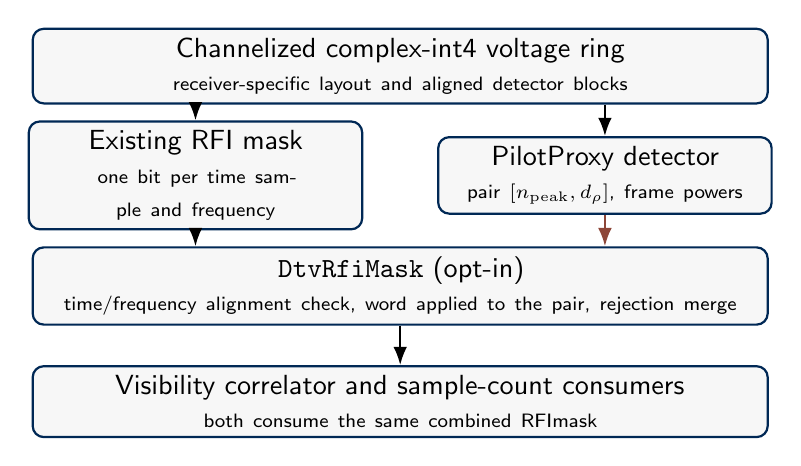
\begin{tikzpicture}[node distance=0.5cm,>=Latex,
  blk/.style={rectangle,rounded corners,draw=PilotProxyBlue,thick,fill=LightGray,
              minimum height=0.75cm,align=center,text width=4.0cm},
  wide/.style={blk,text width=9.1cm}]

\node[wide] (voltage) {Channelized complex-int4 voltage ring\\
  \scriptsize receiver-specific layout and aligned detector blocks};
\node[blk] (rfi) at ($(voltage.south)+(-2.6,-0.9)$)
  {Existing RFI mask\\ \scriptsize one bit per time sample and frequency};
\node[blk] (detector) at ($(voltage.south)+(2.6,-0.9)$)
  {PilotProxy detector\\ \scriptsize pair $[n_{\mathrm{peak}},d_\rho]$, frame powers};
\node[wide,below=1.8cm of voltage] (combine)
  {\texttt{DtvRfiMask} (opt-in)\\
   \scriptsize time/frequency alignment check, word applied to the pair, rejection merge};
\node[wide,below=of combine] (consumers)
  {Visibility correlator and sample-count consumers\\
   \scriptsize both consume the same combined RFImask};

\draw[->,thick] (voltage.south -| rfi.north) -- (rfi.north);
\draw[->,thick] (voltage.south -| detector.north) -- (detector.north);
\draw[->,thick] (rfi.south) -- (combine.north -| rfi.south);
\draw[->,thick,PilotProxyRed] (detector.south) -- (combine.north -| detector.south);
\draw[->,thick] (combine) -- (consumers);
\end{tikzpicture}

\caption{Mask path in Kotekan. The detector reads the voltage ring and writes
a rejection byte, frame powers and rank support for each block.
\code{DtvRfiMask} merges them with the existing RFImask, and the visibility
correlator and the sample-count consumer read the same combined mask. On the
CHIME upgrade there is no \code{DtvRfiMask}, and the detector runs detect
only.}
\label{fig:system_context}
\end{figure}

\subsection{Two loops}

The design has a real-time loop and an offline loop
(Figure~\ref{fig:loops}). The real-time loop applies a fixed bundle to every
block. The offline loop makes the next bundle from data recorded by the
real-time loop. The two loops share one arithmetic, so a word found offline
is the word the stage applies to the same voltages
(\code{src/pilot_proxy/bundle_calibration.py}).

\begin{figure}[H]
\centering
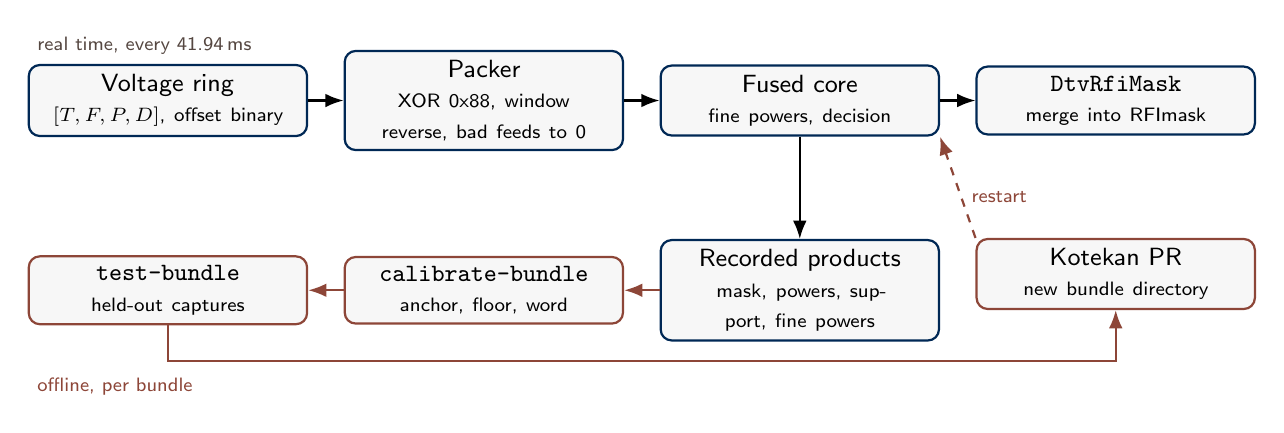
\begin{tikzpicture}[node distance=0.45cm,>=Latex,
  blk/.style={rectangle,rounded corners,draw=PilotProxyBlue,thick,fill=LightGray,
              minimum height=0.8cm,align=center,text width=3.3cm,font=\small},
  off/.style={blk,draw=PilotProxyRed}]
\node[blk] (ring) {Voltage ring\\\scriptsize \([T,F,P,D]\), offset binary};
\node[blk,right=of ring] (pack) {Packer\\\scriptsize XOR 0x88, window reverse, bad feeds to 0};
\node[blk,right=of pack] (core) {Fused core\\\scriptsize fine powers, decision};
\node[blk,right=of core] (fold) {\code{DtvRfiMask}\\\scriptsize merge into RFImask};
\node[blk,below=1.3cm of core] (rec) {Recorded products\\\scriptsize mask, powers, support, fine powers};
\node[off,left=of rec] (cal) {\code{calibrate-bundle}\\\scriptsize anchor, floor, word};
\node[off,left=of cal] (test) {\code{test-bundle}\\\scriptsize held-out captures};
\node[off,below=1.3cm of fold] (pr) {Kotekan PR\\\scriptsize new bundle directory};
\draw[->,thick] (ring) -- (pack);
\draw[->,thick] (pack) -- (core);
\draw[->,thick] (core) -- (fold);
\draw[->,thick] (core) -- (rec);
\draw[->,thick,PilotProxyRed] (rec) -- (cal);
\draw[->,thick,PilotProxyRed] (cal) -- (test);
\draw[->,thick,PilotProxyRed] (test.south) -- ++(0,-0.45) -| (pr.south);
\draw[->,thick,PilotProxyRed,dashed] (pr.north west) -- node[right,font=\scriptsize,pos=0.4]{restart} (core.south east);
\node[font=\scriptsize,PilotProxyGray,anchor=south west] at (ring.north west) {real time, every 41.94\,ms};
\node[font=\scriptsize,PilotProxyRed,anchor=north west] at ($(test.south west)+(0,-0.55)$) {offline, per bundle};
\end{tikzpicture}
\caption{The real-time loop (blue) and the offline loop (red). The detector
reads a new bundle only at a restart. The offline loop is described step by step in the
User Guide and in \code{docs/RUNNING_THE_DETECTOR.md}.}
\label{fig:loops}
\end{figure}

\subsection{Deployment model}

Every node runs the same software and reads the same bundle. At the first
voltage frame, the detector reads the \code{coarse_freq} metadata of the
frame and binds each local frequency to the bundle profile with the same
\code{receiver_channel_id}. A frequency with no profile is not evaluated, and
its mask and powers are zero. A node with no bound profile logs
\code{detector DISABLED (emitting all-zero masks)}. A change of the frequency
order after binding stops the stage.

\begin{itemize}
  \item \textbf{CHORD Pathfinder.} \code{config/chord/pathfinder.j2} includes
        \code{config/chord/dtv.j2} on every X-engine node. The products are
        sent to the recv node and written there (\code{config/chord/recv.j2}).
        REST endpoints switch the mask and the recording until the next
        restart.
  \item \textbf{CHIME upgrade.} \code{config/chime/chime_upgrade_2numa.j2}
        includes \code{config/chime/dtv.j2} in each NUMA domain when
        \code{dtv_enabled} is set. No visibility or weight consumer reads the
        outputs. There is no REST switch.
\end{itemize}

%=====================================================================
\section{Signal Path and Method}
%=====================================================================

\subsection{Signal model}

An ATSC 1.0 8-VSB channel occupies 6\,MHz. Its data shelf is spread over most
of the channel. Its pilot is a narrow tone 309.441\,kHz above the lower channel
edge. ATSC A/53 Part~2 places the pilot about 11.3\,dB below the average data
power \cite{atsc_a53_part2_2011}, and the receiver profiles record this as
\field{pilot_below_data_db} = 11.3. A shelf below the noise floor in a coarse
channel still puts a measurable tone in one fine bin, so the pilot serves as
a proxy for the shelf (Figure~\ref{fig:spectrum_definitions}). U.S. channel 14
spans 470--476\,MHz and channel 36 spans 602--608\,MHz \cite{ecfr_73603}.
Channel 37 (608--614\,MHz) is reserved for radio astronomy and carries no DTV,
so it is the control.

\begin{figure}[H]
\centering
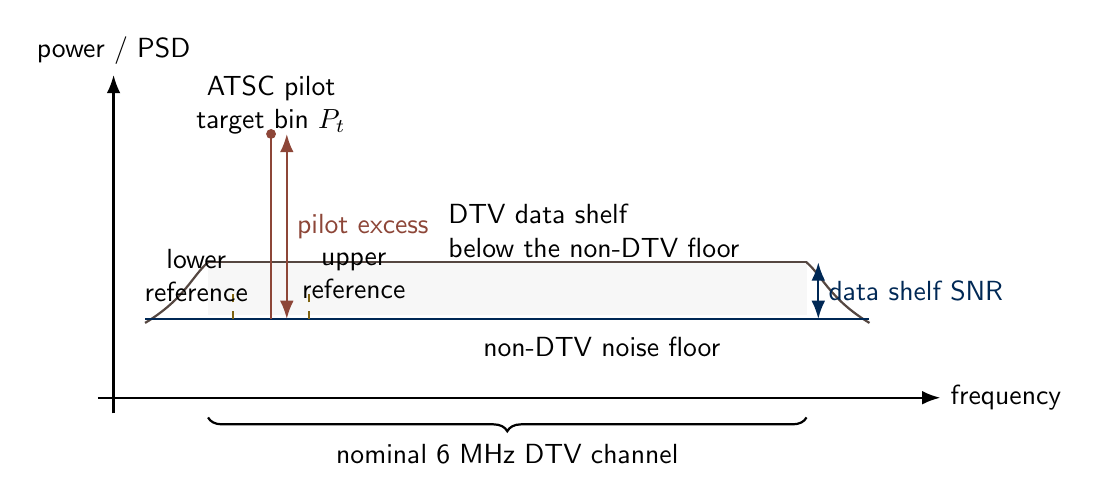
\begin{tikzpicture}[x=1.0cm,y=1.0cm,>=Latex]
  \draw[->,thick] (-0.2,0) -- (10.5,0) node[right]{frequency};
  \draw[->,thick] (0,-0.2) -- (0,4.1) node[above]{power / PSD};
  \draw[fill=LightGray,draw=none] (1.2,1.05) rectangle (8.8,1.72);
  \draw[thick,PilotProxyGray] (1.2,1.72) -- (8.8,1.72);
  \draw[thick,PilotProxyGray] (0.4,0.95) .. controls (0.9,1.25) and (1.0,1.55) .. (1.2,1.72);
  \draw[thick,PilotProxyGray] (8.8,1.72) .. controls (9.0,1.55) and (9.1,1.25) .. (9.6,0.95);
  \draw[thick,PilotProxyBlue] (0.4,1.0) -- (9.6,1.0);
  \draw[thick,PilotProxyRed] (2.0,1.0) -- (2.0,3.35);
  \draw[fill=PilotProxyRed,draw=PilotProxyRed] (2.0,3.35) circle (0.055);
  \draw[dashed,thick,WarnGold] (1.52,1.0) -- (1.52,1.35);
  \draw[dashed,thick,WarnGold] (2.48,1.0) -- (2.48,1.35);
  \draw[<->,thick,PilotProxyRed] (2.20,1.0) -- (2.20,3.35) node[midway,right]{pilot excess};
  \draw[<->,thick,PilotProxyBlue] (8.95,1.0) -- (8.95,1.72) node[midway,right]{data shelf SNR};
  \draw[decorate,decoration={brace,mirror,amplitude=5pt},thick] (1.2,-0.25) -- (8.8,-0.25)
    node[midway,below=6pt]{nominal 6 MHz DTV channel};
  \node[align=center] at (2.0,3.72) {ATSC pilot\\target bin $P_t$};
  \node[align=center] at (1.05,1.55) {lower\\reference};
  \node[align=center] at (3.05,1.55) {upper\\reference};
  \node[align=left] at (6.1,2.12) {DTV data shelf\\below the non-DTV floor};
  \node[align=left] at (6.2,0.65) {non-DTV noise floor};
\end{tikzpicture}
\caption{Signal definitions. The target term sits on the pilot, and the two
reference terms sample the local floor on either side.}
\label{fig:spectrum_definitions}
\end{figure}

\subsection{Geometry}
\label{ssec:geometry}

The detector sees one coarse channel at a time. It cuts each input stream of
the channel into windows of \(K\) samples. One window gives one complex sample
per weight term, so the window rate is the coarse sample rate divided by
\(K\). The detector bin width equals that rate. Both telescopes give the same
detector bin width and the same block length
(Table~\ref{tab:geometry}).

\begin{table}[H]
\centering
\small
\begin{tabular}{|l|r|r|r|}
\hline
\textbf{Quantity} & \textbf{CHIME} & \textbf{CHORD} & \textbf{Pathfinder}\\ \hline
Receiver profile & \code{chime_dtv_fengine} & \code{chord_dtv_fengine} & \code{chord_pathfinder_dtv_fengine}\\ \hline
ADC rate, PFB size & 800\,MS/s, 2048 & 3200\,MS/s, 16384 & 3200\,MS/s, 16384\\ \hline
Coarse channel width & 390625\,Hz & 195312.5\,Hz & 195312.5\,Hz\\ \hline
Nyquist zone, axis order & 2, descending & 1, ascending & 1, ascending\\ \hline
Window \(K\) & 128 & 64 & 64\\ \hline
Detector bin & 3051.76\,Hz & 3051.76\,Hz & 3051.76\,Hz\\ \hline
Block (128 windows) & 16384 samples & 8192 samples & 8192 samples\\ \hline
Block length & 41.94\,ms & 41.94\,ms & 41.94\,ms\\ \hline
Input streams & 2048 & 1024 & 128\\ \hline
Channel ID namespace & \code{chime_freq_id} & \code{chord_freq_id} & \code{chord_freq_id}\\ \hline
Profile status & verified 2026-07-29 & example & example\\ \hline
\end{tabular}
\caption{Geometry of the checked-in receiver profiles
(\code{configs/receiver_profiles/}). ``Example'' is the profile status
\code{example_requires_data_product_verification}.}
\label{tab:geometry}
\end{table}

The padded transform over the 128 windows of a block has \ppFineNumBins\ bins
of \ppFineBinHz\,Hz, which span one detector bin. For CHIME, \code{freq_id}
\(=\) \code{coarse_channel_index} \(+1\), and the channel-14 pilot is in
\code{freq_id} 844.

\subsection{Stage 1: matched filter}

Each bundle profile holds three packed int4 weight vectors of \(K\) taps: the
target, centered on the nominal pilot, and the lower and upper references.
For weight term \(n\) and detector row \(m\) (one window of one stream), the
core forms the exact complex dot product
\begin{equation}
  z[n,m]=\sum_{k=0}^{K-1} x_m[k]\,\overline{w_n[k]},
\end{equation}
in \code{int32} components. In signal-processing terms, stage 1 is a
critically sampled DFT filterbank with a rectangular one-tap prototype,
evaluated only at three channels. The reference terms are
\field{reference_offset_bins} = 2 detector bins from the target, with
\field{skipped_guard_bins} = 1 bin left between them.

\subsection{Stage 2: fixed-point fine transform}

The rows of each term are reshaped to \([N_\text{streams}, 128]\). The frozen
fixed-point transform \code{fxfft256_v1} (zero padding 128 to 256, Q15
twiddles, rounding \(\lfloor(v+2^{14})/2^{15}\rfloor\)) is applied along the
window axis, and the squared magnitudes are summed over streams:
\begin{equation}
  S[n,b]=\sum_{s}\bigl|\mathrm{fxfft256}(z[n,s,\cdot])[b]\bigr|^2
  \qquad(\text{exact \code{uint64}}).
\end{equation}
The sum is coherent in time over one block and incoherent over streams. The
transform is the second stage of a two-stage zoom channelizer, and it refines
the detector bin to the fine bin (Figure~\ref{fig:detector_datapath}).

No phase corrector is needed between windows. The steering frequency of each
term is an integer detector bin, so the phase of an offset tone advances by an
integer number of turns per window through stage~1. The rectangular window
of stage~1 gives the capture factor \(\mathrm{sinc}^2(\delta f/
\ppDetectorBinHz\,\mathrm{Hz})\), a loss of \ppCaptureLossThreeHundredDb\,dB
at 300\,Hz and \ppCaptureLossFiveHundredDb\,dB at 500\,Hz
(\code{docs/METHOD_SPEC.md}). The scalloping loss is at most
\ppCaptureLossEdgeDb\,dB at the edge of the fine span.

\begin{figure}[H]
\centering
% Detector datapath in the two-stage channelizer (filterbank) view.
% This file is the one source of the diagram. It is \input by PilotProxy_DD001
% (Design Document) and PilotProxy_UG001 (User Guide), and
% detector_datapath_standalone.tex renders it to detector_datapath.svg for
% Markdown. It needs the tikz libraries arrows.meta, positioning, calc and
% decorations.pathreplacing, and the colors PilotProxyBlue, PilotProxyRed,
% PilotProxyGray and LightGray from the host document or the standalone
% wrapper. The svg must be rendered again after each edit:
%   cd docs/figures && pdflatex detector_datapath_standalone.tex \
%     && pdftocairo -svg detector_datapath_standalone.pdf detector_datapath.svg
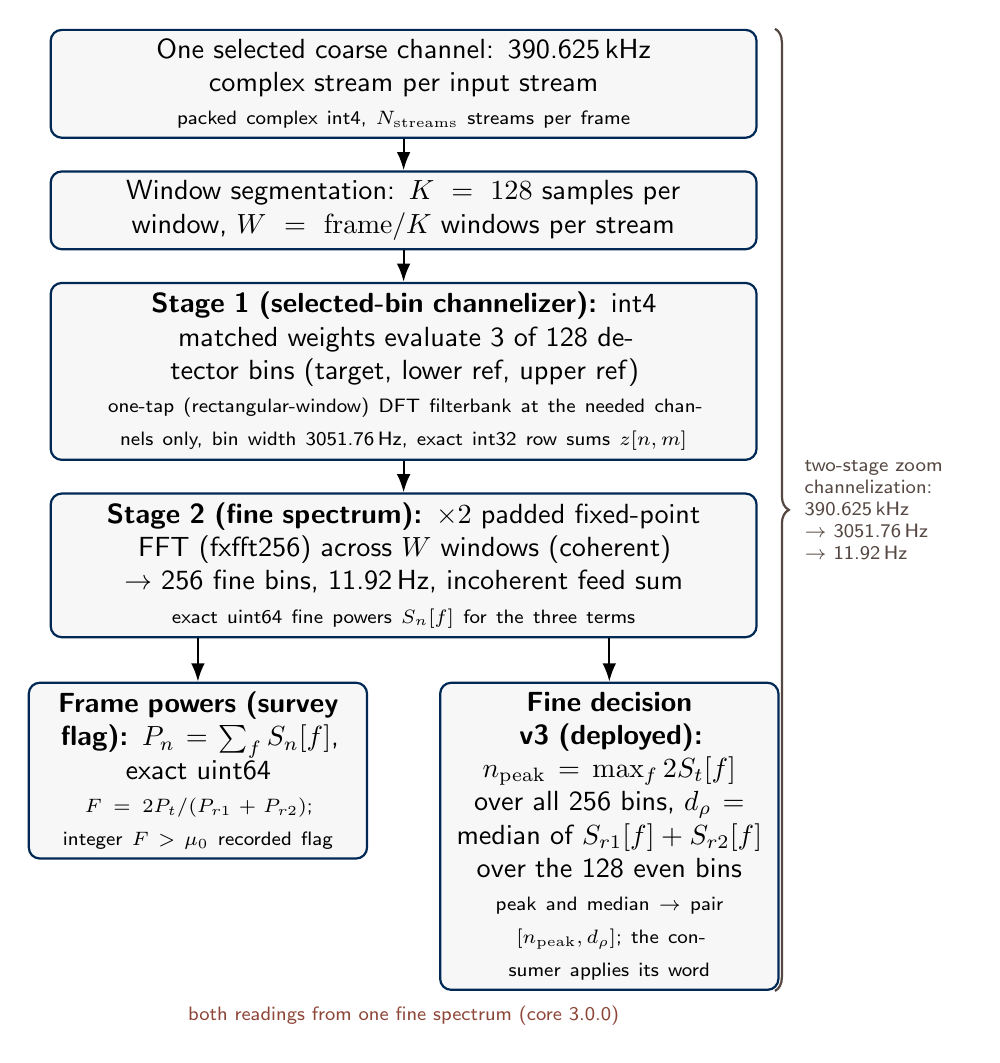
\begin{tikzpicture}[node distance=0.40cm,>=Latex,
  blk/.style={rectangle,rounded corners,draw=PilotProxyBlue,thick,fill=LightGray,
              minimum height=0.62cm,align=center,text width=0.72\linewidth},
  half/.style={rectangle,rounded corners,draw=PilotProxyBlue,thick,fill=LightGray,
               minimum height=0.62cm,align=center,text width=0.335\linewidth}]

\node[blk] (in) {One selected coarse channel: 390.625\,kHz complex stream
  per input stream\\ \scriptsize packed complex int4,
  $N_{\mathrm{streams}}$ streams per frame};
\node[blk,below=of in] (seg) {Window segmentation: $K=128$ samples per
  window, $W=\mathrm{frame}/K$ windows per stream};
\node[blk,below=of seg] (s1) {\textbf{Stage 1 (selected-bin
  channelizer):} int4 matched weights evaluate 3 of 128 detector bins
  (target, lower ref, upper ref)\\ \scriptsize one-tap
  (rectangular-window) DFT filterbank at the needed channels only,
  bin width 3051.76\,Hz, exact int32 row sums $z[n,m]$};
\node[blk,below=of s1] (s2) {\textbf{Stage 2 (fine spectrum):}
  $\times 2$ padded fixed-point FFT (fxfft256) across $W$ windows
  (coherent) $\to$ 256 fine bins, 11.92\,Hz, incoherent feed sum\\
  \scriptsize exact uint64 fine powers $S_n[f]$ for the three terms};
\node[half,anchor=north east] (v1) at ($(s2.south)+(-0.45,-0.55)$)
  {\textbf{Frame powers (survey flag):} $P_n=\sum_f S_n[f]$, exact
  uint64\\ \scriptsize $F = 2P_t/(P_{r1}+P_{r2})$; integer $F>\mu_0$
  recorded flag};
\node[half,anchor=north west] (v2) at ($(s2.south)+(0.45,-0.55)$)
  {\textbf{Fine decision v3 (deployed):}
  $n_{\mathrm{peak}}=\max_f 2S_t[f]$ over all 256 bins,
  $d_\rho=$ median of $S_{r1}[f]+S_{r2}[f]$ over the 128 even bins\\
  \scriptsize peak and median $\to$ pair $[n_{\mathrm{peak}},d_\rho]$;
  the consumer applies its word};

\draw[->,thick] (in) -- (seg);
\draw[->,thick] (seg) -- (s1);
\draw[->,thick] (s1) -- (s2);
\draw[->,thick] (s2.south -| v1.north) -- (v1.north);
\draw[->,thick] (s2.south -| v2.north) -- (v2.north);
\node[font=\scriptsize\color{PilotProxyRed},align=center]
  at ($(s2.south |- v2.south)+(0,-0.32)$)
  {both readings from one fine spectrum (core 3.0.0)};

\coordinate (brx) at ([xshift=0.22cm]s1.east);
\draw[decorate,decoration={brace,amplitude=5pt},thick,PilotProxyGray]
  (brx |- in.north) -- (brx |- v2.south)
  node[midway,right=7pt,font=\scriptsize\color{PilotProxyGray},align=left,
       text width=2.0cm]
  {two-stage zoom channelization:\\ 390.625\,kHz\\ $\to$ 3051.76\,Hz\\
   $\to$ 11.92\,Hz};
\end{tikzpicture}

\caption{Detector datapath. Stage 1 is a filterbank evaluated at three
channels through the int4 weights. The window-axis transform is the second
stage of a zoom channelizer. The frame powers and the fine decision both come
from the same fine spectrum.}
\label{fig:detector_datapath}
\end{figure}

\subsection{Frame powers and the coarse ratio}

The frame power of each term is the sum of its fine spectrum:
\begin{equation}
  P_n=\sum_{b=0}^{255}S[n,b],\qquad
  F=\frac{2P_t}{P_l+P_u}.
\end{equation}
Under a flat noise floor, the expected ratio is set by the integer weight
norms:
\begin{equation}
  \mu_0=\frac{2\lVert w_t\rVert^2}{\lVert w_l\rVert^2+\lVert w_u\rVert^2},
\end{equation}
stored as \field{null_power_ratio}. Int4 rounding makes the norms unequal, and
\(\mu_0\) ranges from \ppMuZeroMin\ to \ppMuZeroMax\ over the
\ppWeightChannelCount\ channels of the shipped bank. The archive products set
\field{reject_mask} by the exact host comparison
\begin{equation}
  \text{valid}=(P_l+P_u\neq0),\qquad
  \text{mask}=\text{valid}\wedge
  \bigl(P_t\,(\lVert w_l\rVert^2+\lVert w_u\rVert^2)>\lVert w_t\rVert^2(P_l+P_u)\bigr),
\end{equation}
which is \(F>\mu_0\) without a division. The bundle records the same rule as
the rational \field{positive_excess_half_threshold_num} :
\field{positive_excess_half_threshold_den}. This coarse rule is a diagnostic.
The deployed decision is the fine rule below.

\subsection{Fine decision v1}
\label{ssec:fine_decision}

The fine statistic at bin \(b\) is
\begin{equation}
  F_2[b]=\frac{2S_t[b]}{S_l[b]+S_u[b]}.
\end{equation}
The bundle supplies, per channel, an anchor bin \(a\), a designated
half-width \(h\), a 256-bit bulk mask, a zero-based rank \(r\) and the word
\(c\). The decision is:

\begin{enumerate}
  \item The bulk is the set of bins in the bulk mask with a positive
        denominator.
  \item If the bulk has \(r\) or fewer bins, the frame is invalid, and its mask
        is 0.
  \item \(F_{2,r}\) is the value of rank \(r\) in the ascending bulk values,
        found by counting, so ties give a unique value.
  \item The mask is 1 if some designated bin \(b\in\{(a+k)\bmod256:|k|\le h\}\)
        with a positive denominator has
        \(F_2[b] > (c/2^{16})\,F_{2,r}\).
\end{enumerate}

Every comparison is a 128-bit or 192-bit integer cross product. A frame at
equality is kept. The bulk mask holds the independent bins (every second bin
under pad 2). It excludes census-marked bins, the designated set, and a guard
of \(\max(h,2)\) padded bins around the anchor, which the bundle validator
enforces. The frame powers are not read by
the decision. The Python reference is \code{src/pilot_proxy/fine_decision.py}.

In estimation-theory terms, the rule is an order-statistic CFAR detector with
a scan over the designated bins. The rank estimate of the local floor replaces
a mean or median estimate. The word sets the false-alarm rate, and its value
is measured, not derived (Section~\ref{ssec:calibration}).

\subsection{Null distribution}

Under a flat, circular Gaussian null with independent terms, one row of
equal-norm weights gives \(F_\text{row}\sim F(2,4)\). Summing \(M\) rows before
the ratio gives \(F\sim F(2M,4M)\), with mean \(4M/(4M-2)\to1\). Each fine bin
over \(N_s\) streams gives \(F_2[b]\sim F(2N_s,4N_s)\) on independent bins. The
real detector has unequal norms, correlated inputs, a fixed-point transform
and a rank normalization, so none of these laws sets its false-alarm rate. The
names \emph{power ratio} and \emph{rank-based fine score} are used for that
reason (\code{docs/TERMINOLOGY.md}). The floor is measured on a control
channel or on simulated noise.

\subsection{Calibration of the word}
\label{ssec:calibration}

\code{pilot-proxy calibrate-bundle} reads a plan and writes a sealed bundle
and a report (\code{src/pilot_proxy/bundle_calibration.py}). It reads the
captures of each channel with the deployed integer path. The constants below
are module constants of that file.

\begin{itemize}
  \item \textbf{Search.} \(h=32\), so 65 designated bins
        (\code{SEARCH_HALF_WIDTH}).
  \item \textbf{Rank.} The zero-based median of the bulk,
        \((|\text{bulk}|-1)/2\) in integer division. With no excluded bins
        this is 47.
  \item \textbf{Anchor.} The bin of the largest 90th-percentile \(F_2\) within
        \(\pm30\) bins of the nominal bin. It counts as measured when the
        frames above the floor are unlikely under the null (binomial upper
        tail below \(10^{-4}\)). Otherwise the nominal bin is used.
  \item \textbf{Floor.} The \code{null_quantile} (default 0.99) of null scores.
        The scores are peaks over pseudo-searches at bins clear of the real
        search, in control-channel frames or in simulated white noise over
        \code{num_inputs} streams.
  \item \textbf{Knee.} Each frame has a smallest keeping word. The kept
        fraction against \(\log(\text{word})\), with each capture given equal
        weight, bends where the frames with a pilot begin. The knee is the
        word of largest height above the chord of that curve.
  \item \textbf{Word.} The knee, unless the plan sets a word, the pilot was not
        seen, fewer than 30 captures were read, the estimated pilot share is
        above 0.9, or the knee is below the floor. In each of these cases the
        floor is used. The report states the case in \code{word_source}.
  \item \textbf{Power-limit word.} With \code{"threshold": "power_limit"}, the
        word keeps the most frames while the upper residual power meets a
        checked limit from an RFIsher channel table. A channel with no passing
        word holds the floor, and \code{bundle.decisions.json} records the
        outcome for the operating-policy compiler.
\end{itemize}

\code{pilot-proxy test-bundle} then checks the bundle on other captures:
structure and digests, values on every bound channel, no shared captures with
calibration, rank support per channel, the masked fraction against the
calibration interval, and the false-alarm count on the control.

%=====================================================================
\section{Design Choices}
\label{sec:choices}
%=====================================================================

Each subsection gives the choice, the reason and the limits. The archive
measurements quoted here are from \code{docs/DESIGN_DECISIONS.md}.

\subsection{Exact integer arithmetic end to end}
\choice{Every quantity from the packed sample to the mask bit is an exact
integer. The fine transform is fixed point and frozen as \code{fxfft256_v1},
with golden vectors in \code{tests/data/fxfft256_golden_v1.npz}.}
{Float FFTs, medians and interpolated quantiles cannot be made bit-exact
across numpy, nvcc and compiler versions. With exact integers, the Python
reference, the CPU model and the GPU give the same bits, a mask can be
recomputed offline from stored powers, and any test failure is a real
difference.}
{The rounded transform does not conserve energy exactly. The departure is
bounded by a factor of 1.001 at full scale (\code{cuda/config.h}) but reaches
tens of percent for unit-amplitude rows. A new transform is a new detector
contract.}

\subsection{\texorpdfstring{$K=128$}{K=128} for CHIME and \texorpdfstring{$K=64$}{K=64} for CHORD}
\choice{One CUDA source compiles for \(K=64\) or \(K=128\). CHIME uses 128,
CHORD and the Pathfinder use 64. Both keep 128 windows per block.}
{CHIME channels are 390.625\,kHz wide and CHORD channels 195.3125\,kHz, so
these values give the same 3051.76\,Hz detector bin, the same 41.94\,ms block
and the same frozen 256-bin fine transform. \(K=128\) also matches the CHIME
manifest and the regression data.}
{The int4 growth bound admits \(K\le128\): one 128-tap component reaches
\(2^{14}\), and 256 taps would exceed signed 16 bits. \(K=256\) is not
implemented. It would need its own fixed-point bound, weight bank, contract and
validation. \(K=512\) is not a candidate.}

\subsection{Frame powers are the sums of the fine powers}
\choice{\(P_n=\sum_bS[n,b]\). Product schema v6 and detector contract
revision~2 (\code{coarse_power_definition = sum_of_fxfft256_fine_powers}) fix
this definition. It holds from kernel core 3.0.0.}
{The coarse ratio and the fine statistic are two readings of one spectrum. One
measurement path needs validation, and no identity between paths has to be
enforced. A row-domain sum \(\sum_m|z|^2\) agrees only to the rounding of the
transform: a median relative \(2.75\times10^{-6}\) on archive frames, and up
to about 2 percent on near-empty frames.}
{The schema v5 products of record store row-domain powers. Readers recompute
the v6 powers from the stored \code{fine_power_u64}. Over 770474 archive
frames this changes \code{reject_mask} on 50 frames, each within
\(7\times10^{-6}\) of the boundary, and changes no threshold-rule outcome. The
host applies the coarse rule in exact integers, because \(P_t\) times the
denominator does not fit \code{uint64} at this scale.}

\subsection{The norm-corrected coarse rule}
\choice{The archive flag compares each channel with its own
\(\mu_0\) instead of 1.}
{Int4 weights leave the target and reference norms unequal. A common
threshold at \(F=1\) would put channels on different sides of their own null
points. The corrected rule is defined by the shipped weights alone, has no
fitted threshold, and is reproducible from integer powers.}
{The rule sets no false-alarm rate. At \(\mu_0\) it holds a detection
probability near 1 but discards 48.5\% of verified-quiet time by construction.
Products record their rule in \code{mask_rule}.}

\subsection{The fine designated-set CFAR is the deployed decision}
\choice{The deployed decision is fine decision v1 (Section~\ref{ssec:fine_decision}).}
{The receiver operating characteristic was measured on the archive. The
coarse null bulk and the weak-signal bulk overlap almost completely, so each
coarse operating point either discards about half the clean time or misses
most weak-channel detections (Table~\ref{tab:roc}). The coherent window sum
recovers up to \ppCoherentGainDb\,dB of deflection over the coarse reduction
(\(10\log_{10}\sqrt{W}\) for \(W=128\)). On the same frames, the fine
designated set reached \(P_d\approx0.99\) on all three channels at a measured
\(P_\text{fa}\) of 0.091, with the \(\pm2\)-bin set and an uncalibrated
multiplier.}
{The null in Table~\ref{tab:roc} is a transmitter-off epoch inferred from the
archive (the ch35 off state, \(n=66\)), not a verified signal-free population.
A deployment false-alarm limit must come from a verified null of the band
itself. In the archive product contract the fine decision stays inactive
(\code{fine_candidate_decision.active = false}). Changing that is a schema
revision at a survey epoch boundary.}

\begin{table}[H]
\centering
\small
\begin{tabular}{|c|c|c|c|c|}
\hline
\(P_\text{fa}\) (null quantile) & \(\theta=F/\mu_0\) & ch36 \(P_d\) & ch35 \(P_d\) & ch34 \(P_d\)\\ \hline
0.10 (P90) & 1.114 & 0.904 & 0.996 & 0.099\\ \hline
0.05 (P95) & 1.124 & 0.872 & 0.996 & 0.089\\ \hline
0.015 (null max) & 1.146 & 0.805 & 0.996 & 0.071\\ \hline
\end{tabular}
\caption{Coarse operating points on the archive. Null: ch35 off state
(\(n=66\)). Signal: on-epochs from 2024 of channels 34 to 36. From
\code{docs/DESIGN_DECISIONS.md}; the ROC evidence is in
\code{docs/evidence/youden_j_2026-09-07/}.}
\label{tab:roc}
\end{table}

\subsection{A rank, not a location and scale}
\choice{The floor estimate is an order statistic of the bulk.}
{It is exact and reproducible on every platform. Order statistics reject the
measured 0.29\% bulk tail by construction, so no contamination fallback mode
is needed. It can be rescored offline from the stored \code{fine_power_u64}
terms.}
{The rank and the bulk set the effective null law, so a word belongs to its
geometry. A word moved from another record must come with its anchor, search
and reference bins. The archive characterization used rank 62 (\(\rho=63\);
60 on channel 20 and 53 on channel 34) with its 125- or 126-bin bulk. That
pair is an experimental profile of its own and is not a requirement of a
runtime bundle (\code{docs/OPERATOR_HANDOFF.md}).}

\subsection{The 65-bin search}
\choice{\code{calibrate-bundle} writes \(h=32\), so 65 designated bins. The
archive characterization and the default export block used \(h=2\)
(\code{FINE_CALIBRATION_DEFAULT_HALF_WIDTH}, ``survey window convention'').}
{On the reserved captures, a copy of the channel-32 pilot lay 238\,Hz from
nominal, outside the five-bin search, and the frames that search kept carried
the excess of the whole capture. The wider search was adopted after those
captures were inspected (dissertation, \code{chapters/conclusions.tex}).}
{The choice is retrospective, and no independent data have tested it. A
scattered line 519\,Hz from nominal in the second reserved capture lies outside
its reach. The null score is a maximum over the search, so a wider search raises the floor.}

\subsection{One fused kernel}
\choice{\code{PilotProxy_Compute_FusedFineMask_U64} goes from packed samples
to one mask bit per block in one launch, with one CUDA block per stream. The
row sums stay in shared memory, and the fine transform runs in place. A
last-block epilogue forms the decision, with the completion counter folded
into the mask element (fence, then atomic).}
{The row sums never touch global memory in production. The butterflies of
one stage write disjoint pairs, and every sum is an exact integer, so the
result does not depend on the thread schedule. The governing rule is bit
identity with the frozen reference and the golden vectors.}
{The row sums are exposed only through an optional debug tap. On an A100 with
core 2.3.0, the fused form took 0.769\,ms per 2048-stream block and the mask
form 0.895\,ms, of which the epilogue was 0.127\,ms, against the 41.94\,ms
cadence. The repository records no timing for core 4 or for the deployment
GPUs, and \code{docs/RUNNING_THE_DETECTOR.md} checks the time per block from
\code{/gpu_profile} on each run.}

\subsection{Guard and reference names}
\choice{The public terms are \field{skipped_guard_bins} and
\field{reference_offset_bins}, with \code{reference_offset_bins =
skipped_guard_bins + 1}.}
{One name per quantity. A user-written core profile gives
\field{skipped_guard_bins}, and generated metadata records both so the
geometry can be audited. \code{scripts/check_no_legacy_guard_terms.sh} rejects
the retired names.}
{The core compiles \code{PILOTPROXY_REFERENCE_BIN_OFFSET = 2}. A different
offset needs a new weight bank.}

\subsection{Adaptive, recorded reference placement}
\choice{The weight generator keeps the requested reference offset when the
receiver geometry allows it. A reference past the baseband-frame origin
wraps. A reference that would land on the forbidden coarse-channel DC tone
moves away. A target on DC is an error.}
{Moving the target would change the signal under test, while a reference can
move without changing the test. Products and manifests record the placement,
so later analyses read it instead of reconstructing it.}
{In the shipped bank for channels 14 to 36, channel 14 is the only adaptive
case: its lower reference wraps across the coarse-channel center, with the DC
tone in the skipped guard. No shipped channel collides with DC. The upper
reference of channel 21 crosses the coarse-channel half-width and samples the
channelizer roll-off, and the manifest marks it as crossing.}

\subsection{The bundle is the interface}
\choice{Kotekan reads five files from a local directory once, at startup, and
checks every digest. A bundle is never edited. Each one is a directory named
\code{<purpose>-<first 8 hex digits of the SHA-256 of sha256sums.txt>}, added
to Kotekan by a pull request.}
{The arithmetic is code and the operating point is data, so a recalibration
changes no code and no schema. A lookup service at startup could stop the
correlator along with the detector. The digest in the name ties a deployed
run to its numbers.}
{A bundle changes only at a restart. A valid bundle shows only that it is
well formed. Schema validation says nothing about the quality of a
calibration.}

\subsection{The word is fixed during a run}
\choice{The word does not follow the live data. The live data feed the next
bundle, which is tested before it is deployed.}
{A threshold that followed the data would rise with a stronger pilot and stop
masking it, and the kept data would have no fixed definition.}
{A pilot that moves out of the designated bins, or a new line in the
reference bins, needs a recalibration and a restart.}

\subsection{Channel 37 is the control}
\choice{Channel 37 can be bound with \code{fine_calibration.status: control}.
Its decisions are formed and recorded, and its mask stays zero. Only channel
37 may carry that status, and it is never \code{calibrated}.}
{The floor needs frames of the same receiver with no pilot. A channel
reserved for radio astronomy gives them under the same gains and inputs.}
{A null on channel 37 does not show a null on every channel. The control
support was added to Kotekan in kotekan\#1874.}

\subsection{Bad feeds are packed as zero}
\choice{With \code{bf_mask_name} set, the packer writes every input flagged by
\code{bufferBadInputs} as zero.}
{A dead or noisy input would otherwise change the noise of the sum. On CHORD,
\code{bufferBadInputs} also flags the RFI antennas.}
{A change in the flagged set changes the noise of the sum. The plan's
\code{num_inputs} is recorded as \code{summed_inputs}, and the detector warns
while the count of good inputs differs from it by more than 10\%. It warns
rather than stops, because feeds are flagged and restored in normal running.
On CHIME, the bad-feed mask is added by kotekan\#1880, which is open.}

\subsection{Detect-only before masking}
\choice{Every bundle made by \code{calibrate-bundle} is a detect-only
commissioning bundle. A bundle masks only when every \code{calibrated} channel
carries a \code{mask_qualification} record, which \code{qualify-bundle} writes
from a passing test report and the name of the person who read it.
\code{DtvRfiMask} refuses to start with the mask on and a detect-only bundle,
and a POST that switches the mask on stops Kotekan. The detector also refuses
words whose provenance carries \code{qualification: archive_review_only}.}
{The detect-only rule was a note in the bundle and the operator's care. A
machine check reads the same file the detector loads. A person, not a tool,
qualifies a bundle, because no test can show that a word catches weak pilots.
Stopping on a POST keeps \code{N2Accumulate}, which records when the mask was
on, from disagreeing with \code{DtvRfiMask}.}
{A bound channel with status \code{pending_campaign} stops the whole Kotekan
instance at its first frame. An uncalibrated channel is dropped from the
bundle or listed in \code{permanent_mask_freq_ids}. A mistaken POST ends the
run.}

\subsection{Stored fine surface is the exact terms}
\choice{Products store \code{fine_power_u64} with shape
\((N,3,\text{fine\_num\_bins})\) and the decision contract scalars. Every
derived quantity (float ratio, CFAR location, scale and threshold, null-bulk
exceedance fraction) is recomputed in post-processing and never written.}
{One stored surface defines every reading of a frame, and a new threshold can
be applied to a recorded run.}
{Products that violate the contract are unsupported and must be regenerated.}

\subsection{Source stamp memoized per process}
\choice{\code{detector_version} embeds a hash of every \code{*.py} under
\code{src/pilot_proxy}, computed once per process.}
{The imported code cannot change during a process. Resume compares the full
stamp and aborts on any change, so a new build needs a clean
\code{--output-dir}. Combine and stacking compare only the geometry tokens.}
{The commit behind a stamp is recovered by recomputing the hash at candidate
checkouts.}

%=====================================================================
\section{Data Contracts}
%=====================================================================

\subsection{Receiver profile}

A receiver profile (\code{pilotproxy_receiver_profile_v1}) describes one
telescope above the kernel boundary. Every field is required, unknown fields
are refused, and there is no implicit frame or zone fallback
(\code{INTEGRATION.md}).

\begin{longtable}{|L{0.30\linewidth}|L{0.62\linewidth}|}
\hline
\textbf{Block} & \textbf{Content}\\ \hline
\endhead
\code{rf_band} & Lower and upper RF edge.\\ \hline
\code{channelizer} & ADC rate, PFB size and taps, response, coarse channel count and center offset, \code{frequency_axis.nyquist_zone} and \code{order}.\\ \hline
\code{framing} & \code{frame_size_samples}: 16384 for CHIME, 8192 for CHORD.\\ \hline
\code{input_streams} & Stream count, stream unit, \code{combine_default = incoherent_power_sum_over_streams}.\\ \hline
\code{quantization} & Adapter output \code{complex_int4_packed_int8}, 4 bits per component.\\ \hline
\code{detector_adapter} & \(K\), \code{fine_bin_enbw_hz}, \code{dtv_bandwidth_hz}, \code{pilot_below_data_db}, \code{pilot_capture_efficiency}, \code{time_reverse_detector_windows_before_kernel}.\\ \hline
\code{baseband_frame} & \code{channel_center_normalized} and \code{physical_dc_normalized}: 0.0 for the verified CHIME DC-centered frame.\\ \hline
\code{metadata.channel_id_map} & Namespace and offset from \code{coarse_channel_index} to the telescope channel ID.\\ \hline
\end{longtable}

\subsection{Detector core profile and detector contract}

The detector core profile
(\code{configs/detector_core/pilotproxy_cuda_local_reference_power_ratio.json},
schema \code{pilotproxy_detector_core_profile_v3}) states the kernel contract:
supported \(K\in\{64,128\}\), 3 weight terms, \field{skipped_guard_bins} = 1,
int4 packed input, \code{uint64} powers and no per-frequency threshold.

The bundle file \code{detector_contract.json}
(\code{pilotproxy_detector_contract_v2}) records the contract of the exported
bank: \(K\), the input coordinate system, the window reversal, the coarse
ratio definition, \code{combine_mode = all_rows_summed_before_ratio}, the
coarse \code{mask_rule} and \code{valid_rule}, and the reference placement
summary. The digest of this object, \code{detector_contract_sha256}, is the
SHA-256 of its canonical JSON (sorted keys, compact separators), not of the
file bytes.

\subsection{Runtime bundle}
\label{ssec:bundle}

\begin{longtable}{|L{0.25\linewidth}|L{0.67\linewidth}|}
\hline
\textbf{File} & \textbf{Content}\\ \hline
\endhead
\code{weights.bin} & Concatenated int8 profiles (\code{concatenated_int8_weight_profiles_v1}), each \([3,K]\) packed complex int4: 384 bytes for \(K=128\). Profiles are contiguous and in table order.\\ \hline
\code{weights.manifest.json} & \code{pilotproxy_runtime_weights_manifest_v1}: receiver profile name and hash, core profile name, channel list, weight shape, \code{weights_sha256}, and the full reference layout of each channel.\\ \hline
\code{pilot_profiles.json} & \code{pilotproxy_runtime_pilot_profiles_v1}: receiver profile ID, namespace, coordinate systems, window reversal, contract and weight digests, and one row per channel.\\ \hline
\code{detector_contract.json} & The detector contract above.\\ \hline
\code{sha256sums.txt} & SHA-256 of the four files above.\\ \hline
\end{longtable}

Each row of \code{pilot_profiles.json} holds the physical channel, the
receiver channel ID and its namespace, the pilot frequency, the coarse channel
center and index, the weight bank index, offset and size, the weight norms,
\field{null_power_ratio}, the coarse half-threshold, the reference placement,
and a \code{fine_calibration} block:

\begin{longtable}{|L{0.30\linewidth}|L{0.62\linewidth}|}
\hline
\textbf{Field} & \textbf{Meaning}\\ \hline
\endhead
\code{status} & \code{pending_campaign}, \code{calibrated}, or \code{control} (channel 37 only).\\ \hline
\code{decision_version} & \code{fine_decision_v1}.\\ \hline
\code{anchor_bin} & Fine bin of the pilot, 0 to 255.\\ \hline
\code{designated_half_width} & \(h\). Designated bins are \(a\pm h\) modulo 256.\\ \hline
\code{bulk_mask_words_hex} & Four \code{0x}-prefixed uint64 words. Bin \(b\) is bit \(b\bmod64\) of word \(\lfloor b/64\rfloor\).\\ \hline
\code{cfar_rank} & Zero-based rank, below the bulk population.\\ \hline
\code{cfar_multiplier_q16} & The word, in \([1,2^{64}-1]\).\\ \hline
\code{marker_guard_bins} & Optional extra guard around the designated set.\\ \hline
\code{provenance} & \code{epochs}, \code{source_product_sha256}, \code{null_quantile}, optional \code{note}, \code{summed_inputs}, \code{mask_qualification} and \code{threshold_selection}. A pending block has empty lists and a null quantile. \code{mask_qualification} holds \code{test_report_sha256} and \code{reviewer}, and only a \code{calibrated} block may carry it. A \code{threshold_selection} carries \code{qualification: archive_review_only}.\\ \hline
\end{longtable}

The validator (\code{validate_runtime_weight_bundle} in
\code{src/pilot_proxy/runtime_bundle.py}) checks the digests, the bindings,
the ranges, and that no designated or guard bin is set in the bulk mask. The
Kotekan command repeats the digest, range and status checks at startup.

\notebox{The calibration blocks of the installed bundles say \code{calibrated}
(or \code{control} on channel 37), but none is a calibration. The status
means the values are filled in, so that Kotekan will bind the channel. It does
not mean the channel is qualified for masking, which is the
\code{mask_qualification} record, and no installed bundle has one. The provenance
note of every row ends ``Detect-only, not a calibration.'' The Pathfinder
words are the floor from a control channel on five spaced files of
2026-10-29, fewer than the 30 captures a knee needs. The
\code{chime-hello-world} words are set in the plan from the archive knees of
record. The \code{chime-first} words are a white-noise floor.}

\begin{table}[H]
\centering
\small
\begin{tabularx}{\linewidth}{|L{0.33\linewidth}|L{0.18\linewidth}|Y|}
\hline
\textbf{Bundle} & \textbf{Channels} & \textbf{Use}\\ \hline
\code{chime-hello-world-d1ed7815} & 29, 35 & First detect-only CHIME run.\\ \hline
\code{chime-first-56005bb7} & 14--36, control 37 & Parameters only, to record data for the first calibration. Word 72260 (\(\eta\approx1.103\)) on every channel, from a white-noise floor over 2048 inputs, \(h=32\), rank 47. Added by kotekan\#1880.\\ \hline
\code{pathfinder-commissioning-b8026807} & 18, 24, 29 & Pathfinder detect-only runs (kotekan\#1862).\\ \hline
\code{pathfinder-commissioning-e2e90219} & 18, 24, 29, control 37 & The same words, and records channel 37 for the next calibration (kotekan\#1877). The default after kotekan\#1895.\\ \hline
\end{tabularx}
\caption{Bundles in Kotekan, from \code{config/chime/dtv_bundles/README.md}
and \code{config/chord/dtv_bundles/README.md}. None qualifies a channel for
masking.}
\label{tab:bundles}
\end{table}

\subsection{Kotekan interfaces}

\code{cudaPilotProxyDetector} reads packed \([T,F,P,D]\) voltages and writes,
per block:

\begin{longtable}{|L{0.22\linewidth}|L{0.24\linewidth}|L{0.46\linewidth}|}
\hline
\textbf{Output} & \textbf{Type and shape} & \textbf{Content}\\ \hline
\endhead
\code{dtv_mask} & int8 \([1,F]\) & 1 = reject. Zero on unbound frequencies and on the control.\\ \hline
\code{dtv_powers} & uint64 \([1,F,3]\) & Target, lower and upper frame powers.\\ \hline
\code{dtv_fine_support} & int32 \([1,F,2]\), optional & \((\text{rank\_valid},n_\text{bulk})\): \((-1,-1)\) not evaluated, \((0,n)\) too few bulk bins, \((1,n)\) valid.\\ \hline
\code{dtv_fine_powers} & uint64 \([1,R,3,256]\), optional & Fine powers of bound channel \(i\) in row \(i\). \code{coarse_freq} names the row, \(-1\) when unused.\\ \hline
\end{longtable}

Its main config keys are \code{detector_window_samples},
\code{receiver_channel_id_namespace}, \code{pilot_profiles_path},
\code{weights_path}, \code{permanent_mask_freq_ids}, \code{bf_mask_name},
\code{dtv_fine_powers_rows} and \code{enabled_updatable_config}. The stage
reference is \code{docs/sphinx/user/modules/pilotproxy.rst} in Kotekan.

\code{DtvRfiMask} reads an RFImask frame (\code{uint1x8}
\([\text{num\_times}/1024,F,128]\), 1 = keep), the detector mask and,
optionally, the support rows. For each frequency it clears every time bit when
the detector rejects, when rank support is invalid, or when the frequency is
in \code{permanent_mask_freq_ids}. \code{require_fine_freq_ids} names
frequencies that must carry an evaluated decision. Any mismatch of time,
frequency, upchannelization or support identity stops the run. It accepts
8192- and 16384-sample blocks. It reads \code{pilot_profiles_path} for the
qualification check above.

\subsection{Products}

\begin{longtable}{|L{0.28\linewidth}|L{0.64\linewidth}|}
\hline
\textbf{Product} & \textbf{Definition}\\ \hline
\endhead
Per-pilot archive product & \code{_per_pilot/<freq_id>.npz}, schema \code{pilotproxy_per_pilot_product_v6}. Fields in \code{docs/PRODUCT_SCHEMA.md}, \code{docs/PER_PILOT_PRODUCT_FIELDS.md} and \code{docs/FINE_REDUCTION_PRODUCTS.md}. The writer, the reader and \code{tools/audit_per_pilot.py} enforce \(P_n=\sum_bS[n,b]\) exactly.\\ \hline
Archive products of record & Schema v5, detector contract v1: \code{chime_pilots_rebuild_20260829} (core 2.3.0) and the channel 37 control \code{ch37_control_491_20260924}. Never edited. Readers recompute the frame powers from \code{fine_power_u64}.\\ \hline
Detect-only run, CHIME & Raw files \code{dtv_mask}, and with \code{dtv_calibration_mode} also \code{dtv_powers} and \code{dtv_fine_support}, 1024 frames per file; HDF5 \code{dtv_fine_powers}, about 43\,s per file, about 2.3\,MB/s per NUMA domain.\\ \hline
Detect-only run, Pathfinder & Files on the recv node under \code{/mnt/cs00/data/dtv/acq_<start time>/}, one per NUMA half and window of about 43\,s.\\ \hline
Calibration outputs & \code{bundle/}, \code{bundle.report.json}, and for the power-limit threshold \code{bundle.decisions.json} (\code{pilotproxy-power-decisions-v4}).\\ \hline
Operating policy & \code{policy.json} from \code{compile-operating-policy}: a finite word, \code{reject_all} or \code{pass_all} per channel, with \code{permanent_mask_freq_ids} and \code{require_fine_freq_ids} for the consumer (\code{docs/CHANNEL_OPERATING_POLICY.md}).\\ \hline
\end{longtable}

Masked frames are dropped from averages and never replaced with zeros.
Resume and combine require the exact schema identity, decision contract,
geometry, timing identity, weights and provenance, and there are no fallback
readers.

\subsection{Data format and fixed-point sizing}

Each input sample is one \code{int8_t}: bits [7:4] are the real part and bits
[3:0] the imaginary part, each two's-complement int4 in \([-8,7]\). The
telescope rings are offset binary, and the packer converts them with XOR
\code{0x88}. Weights use the symmetric range \([-7,7]\). The input matrix is
row-major, \(\mathrm{d\_in}[m,k]=\mathrm{d\_in}[mK+k]\), with the windows of
each stream contiguous.

One complex-product component is bounded by 128, so a 128-tap row sum is
bounded by \(2^{14}\) and fits signed 16-bit storage. The fixed-point
transform stays in \code{int32}. With \(R=128K\), the frame power obeys
\(P_n\le256\cdot2R^2\cdot128\cdot N_\text{streams}\cdot1.001\): about
\(2^{55}\) at 2048 streams and \(2^{60}\) at the asserted capacity of
\(2^{16}\) streams (\code{cuda/config.h}).

\subsection{C API}
\label{ssec:capi}

\small
\begin{longtable}{|L{0.50\linewidth}|L{0.42\linewidth}|}
\hline
\textbf{Function} & \textbf{Purpose}\\ \hline
\endhead
\apicode{PilotProxy_GetSpecs}, \apicode{PilotProxy_GetFineSpecs} & Compiled \(K\), terms, bits and reference offset; fine geometry 128/2/256.\\ \hline
\apicode{PilotProxy_GetFeatures}, \apicode{PilotProxy_GetOptimizationFeatures}, \apicode{PilotProxy_GetVersion} & Build features and the core version.\\ \hline
\apicode{PilotProxy_LastError} & Last error of the calling thread.\\ \hline
\apicode{PilotProxy_Create}, \apicode{PilotProxy_Create_Batch}, \apicode{PilotProxy_Destroy} & Device-affine handle over a packed input buffer.\\ \hline
\apicode{PilotProxy_SetStream} & CUDA stream of the handle (default stream 0).\\ \hline
\apicode{PilotProxy_Compute_RowSums_I32} & Exact int32 row sums, term-major, stream-major rows.\\ \hline
\apicode{PilotProxy_Compute_FinePowers_U64} & Fine powers from a row-sum buffer. Handle-free.\\ \hline
\apicode{PilotProxy_Compute_FusedFine_U64} & Packed samples to fine powers and frame powers in one fused launch.\\ \hline
\apicode{PilotProxy_Compute_FusedFineMask_U64} & Fused launch plus the fine decision v1 epilogue. One mask per block.\\ \hline
\apicode{PilotProxy_Compute_FusedFineMaskWithSupport_U64} & As above, plus \code{rank_valid} and \code{n_bulk}. Used by Kotekan when the support buffer is bound.\\ \hline
\apicode{PilotProxy_Supports_*} & Run-time probes for each compute entry.\\ \hline
\end{longtable}
\normalsize

A handle must not be used by two host threads at once. The caller sets the
CUDA device before creating a handle and keeps it for compute and destroy.
The library forms no ratio and no coarse threshold, and it has no float
helpers since core 3.0.0. Build options are \code{SM}, \code{DP4A} (default
on), \code{DETECTOR_WINDOW_SAMPLES} (default 128), \code{BLOCK_THREADS}
(default 64) and \code{GRID_MAX_BLOCKS} (default 4096) in \code{cuda/Makefile}.

%=====================================================================
\section{Validation}
%=====================================================================

\subsection{How the code is validated}

The validation rests on bit identity. Each layer has a reference that it
must match exactly.

\begin{longtable}{|L{0.25\linewidth}|L{0.67\linewidth}|}
\hline
\textbf{Layer} & \textbf{Check}\\ \hline
\endhead
Fine transform & \code{src/pilot_proxy/fxfft.py} and golden vectors; C, Python and device parity (\code{tests/core/test_fxfft*.py}, \code{tests/kernel/test_fxfft256_gpu.py}).\\ \hline
Decision arithmetic & \code{tests/core/test_fine_decision.py} against a \code{fractions.Fraction} oracle; 128- and 192-bit products fuzzed over 2 million trials against Python integers; 10000 boundary and random cases per GPU build (\code{tests/kernel/test_kernel_matrix_gpu.py}).\\ \hline
Fused kernel & Threaded CPU emulation of the device code, one pthread per CUDA thread, bit-identical for noise, an injected pilot, a wrapped anchor, a degenerate bulk and an unbound tap. On the GPU: \code{tests/kernel/test_fused_fine_gpu.py} and \code{tests/kernel/test_fused_mask_gpu.py}, including last-block determinism over 20 repeats.\\ \hline
Kernel matrix & \(K\) = 64 and 128, scalar and DP4A, weight placements, 32/64/128 threads, restricted grids (\code{tests/kernel/test_kernel_matrix_gpu.py}).\\ \hline
C ABI & \code{cuda/tests/} with the CPU reference (\code{make -C cuda test}).\\ \hline
Bundles & \code{tests/core/test_runtime_bundle.py}, \code{tests/core/test_bundle_calibration.py}; \code{validate-runtime-weight-bundle}; \code{test-bundle} on held-out captures.\\ \hline
Placement & Synthesized pilot and reference tones over channels 14--36, Nyquist zone, edge and DC (\code{tests/core/test_chord_tone_injection.py}, \code{tests/core/test_atsc_channels.py}).\\ \hline
Kotekan & \code{tests/test_pilotproxy_integration.py} against integer CPU references; \code{tests/test_dtv_rfi_mask.py} for visibilities and counts across ring wrap; \code{tests/boost/test_DtvRfiMask.cpp}; \code{tests/ci-scripts/pilotproxy/run_pilotproxy_tests.sh}; the production-geometry soak with 2048 inputs (\code{docs/sphinx/dev/dev_pilotproxy_chime.rst}).\\ \hline
Archive run & The gates of \code{docs/VALIDATION_GATES.md}: clean source, full test tree, CPU reference, pinned library digest, real-file and resume gates.\\ \hline
\end{longtable}

The GPU gate (\code{make test-gpu}) fails when a GPU test skips. The component
map is \code{docs/TEST_COVERAGE.md}. The ground truth of the CHIME frame is
closed: \code{tools/framing_audit.py} reports \code{VERDICT: ALIGNED} for
\code{freq_id} 844, and a parity census over the 23 channels confirmed the
DC-centered bank.

\subsection{Evidence of record}

\begin{itemize}
  \item The archive run of record passed the gates with the preserved core
        2.3.0 library and wrote schema v5 products.
  \item \code{docs/evidence/youden_j_2026-09-07/}: coarse against fine ROC on
        the released products.
  \item \code{docs/evidence/ch37_rank_injection_2026-09-30/}: rank curves and
        real-null exceedance rates of the channel 37 control.
  \item \code{docs/evidence/ca_os_archive_bulk_2026-09-29/}: bulk statistics of
        all 23 channels.
\end{itemize}

These files are CHIME-derived. They need CHIME collaboration clearance before
a public release, and \code{tools/make_code_only_cut.py} makes the cut without
them (\code{CHIME_DERIVED.md}).

\subsection{What is not validated}

\begin{itemize}
  \item No word has been tested on independent telescope data. No channel is
        qualified for masking.
  \item The floor of the first CHIME bundle comes from simulated white noise.
        A real control can sit well above it.
  \item The CHORD and Pathfinder receiver profiles are examples, not verified
        against data products.
  \item Telescope replay with a verified receiver state, Compute Sanitizer and
        a sustained shadow run of the full pipeline have not been done.
  \item The recorded timings are for core 2.3.0 on an A100. The repository
        records none for the deployment GPUs.
  \item Failure recovery and pairwise masking are not covered by
        \code{DtvRfiMask}. Shared pair acceptance is not enforced for CHIME
        \code{N2Accumulate}.
  \item The fine decision does not decode ATSC and does not prove that an
        excess is DTV. Rank support does not cover packet loss, feed health or
        physical calibration.
  \item No test shows that a word catches weak pilots. \code{test-bundle}
        tests the floor on the control and the masked fractions.
  \item The power-limit word is in-sample, and its corrections use an
        assumed normalization from the RFIsher table.
\end{itemize}

%=====================================================================
\section{Code Map}
%=====================================================================

\subsection{PilotProxy}

\small
\begin{longtable}{|L{0.40\linewidth}|L{0.52\linewidth}|}
\hline
\textbf{Path} & \textbf{Content}\\ \hline
\endhead
\code{cuda/pilotproxy_detector.{h,cu}}, \code{cuda/config.h} & C API, kernels, compile-time geometry and bounds.\\ \hline
\code{cuda/pilotproxy_reference.*}, \code{cuda/fxfft256_ref.c} & CPU reference.\\ \hline
\code{src/pilot_proxy/kernel.py} & ctypes wrapper \code{PilotProxyKernel}.\\ \hline
\code{src/pilot_proxy/fxfft.py} & Frozen fixed-point transform.\\ \hline
\code{src/pilot_proxy/fine_decision.py} & Python reference of fine decision v1.\\ \hline
\code{src/pilot_proxy/fine_reduction.py}, \code{product_contract.py} & Fine reduction, frame powers, coarse columns.\\ \hline
\code{src/pilot_proxy/detector_weights.py}, \code{integration/weight_generation.py} & Weight banks and reference placement.\\ \hline
\code{src/pilot_proxy/detector_contract.py} & Detector contract, \(\mu_0\), contract digest.\\ \hline
\code{src/pilot_proxy/runtime_bundle.py} & Bundle export and validation.\\ \hline
\code{src/pilot_proxy/bundle_calibration.py} & \code{calibrate-bundle} and \code{test-bundle}.\\ \hline
\code{src/pilot_proxy/power_limit_word.py} & Power-limit test and control corrections.\\ \hline
\code{src/pilot_proxy/run_plans.py}, \code{process_run.py}, \code{run_spectrogram.py}, \code{run_scores.py} & Run splitting, one-step processing, spectrograms and score caches.\\ \hline
\code{src/pilot_proxy/operating_policy.py} & \code{compile-operating-policy}.\\ \hline
\code{src/pilot_proxy/capture_replay.py} & \code{replay-fine-capture}.\\ \hline
\pathcode{src/pilot_proxy/detectors/narrowband_marker/} & Archive anchors, scores and rescoring.\\ \hline
\code{src/pilot_proxy/characterization/} & Archive threshold rule, score cache, eras.\\ \hline
\code{src/pilot_proxy/archive/}, \code{chime/} & Archive scan, inventory, readers and runners.\\ \hline
\code{src/pilot_proxy/testbench/} & GNU Radio ATSC bench and synthetic validation.\\ \hline
\code{src/pilot_proxy/cli.py} & The \code{pilot-proxy} command.\\ \hline
\code{configs/} & Receiver profiles, core profile, stream maps.\\ \hline
\code{tools/} & Audits, extraction, threshold rule script, doc specs.\\ \hline
\code{tests/} & Python, kernel and archive tests.\\ \hline
\end{longtable}
\normalsize

\subsection{Kotekan}

\small
\begin{longtable}{|L{0.40\linewidth}|L{0.52\linewidth}|}
\hline
\textbf{Path} & \textbf{Content}\\ \hline
\endhead
\code{external/pilotproxy/} & Vendored core and \code{VENDOR.json}.\\ \hline
\code{lib/cuda/cudaPilotProxyDetector.cpp} & Bundle loading, binding, launches.\\ \hline
\code{lib/cuda/cudaPilotProxyPacker.cu} & Ring to detector matrix.\\ \hline
\code{lib/stages/DtvRfiMask.cpp} & Mask fold into the RFImask; qualification check.\\ \hline
\code{config/chord/dtv.j2}, \code{recv.j2}, \code{pathfinder.j2} & CHORD Pathfinder graph.\\ \hline
\code{config/chime/dtv.j2} & CHIME upgrade detector, detect only.\\ \hline
\code{config/*/dtv_bundles/} & Installed bundles.\\ \hline
\code{docs/sphinx/user/modules/pilotproxy.rst} & Stage reference.\\ \hline
\code{docs/sphinx/dev/dev_pilotproxy_*.rst} & CHIME validation and testing.\\ \hline
\code{tests/test_pilotproxy_*.py}, \code{tests/test_dtv_rfi_mask.py} & Integration tests.\\ \hline
\end{longtable}
\normalsize

%=====================================================================
\section{Handover}
%=====================================================================

\subsection{Status}

\importantbox{No channel is qualified for masking. Every bundle in Kotekan is
detect only, and Kotekan refuses to mask with it. A bundle from
\code{calibrate-bundle} is a commissioning bundle. Applied masking needs a
telescope calibration, a passing \code{test-bundle} report with the control,
\code{qualify-bundle}, the shadow acceptance of
\code{docs/OPERATOR_HANDOFF.md}, and only then \code{dtv_apply_mask: true}.}

\subsection{Open work and known limitations}

\begin{itemize}
  \item \textbf{CHIME calibration data.} On Kotekan \code{develop},
        \code{config/chime/dtv.j2} writes no fine powers, so a CHIME run cannot
        yet be calibrated, and every input is summed. kotekan\#1880 adds the
        fine powers, the bad-feed mask, calibration mode and the
        \code{chime-first-56005bb7} bundle. It is open.
  \item \textbf{Vendored core.} Kotekan vendors PilotProxy commit
        \code{afe1c9d}, which predates the name
        \code{post_nyquist_zone_normalization} and so cannot validate the
        shipped bundles. A re-vendor at \code{54ae410}, whose \code{cuda/}
        differs only in comments, is on the Kotekan branch
        \code{pilotproxy-revendor-54ae410}. Re-vendor again at each change to
        the core, after the change is merged in PilotProxy.
  \item \textbf{CHIME has no voltage capture path} of its own on the upgrade,
        so first captures come from the CHIME/FRB baseband system.
  \item \textbf{First CHIME calibration.} Record a detect-only run with the
        control, calibrate, test on another day, and replace the simulated
        floor.
  \item \textbf{Pathfinder thresholds.} A 48\,h run with the control
        calibrates on the first day and tests on the second. A passing bundle
        is then read and qualified with \code{qualify-bundle}.
  \item \textbf{Kotekan qualification check.} The \code{DtvRfiMask}
        refusal and the summed-input warning are on the Kotekan branch
        \code{pilotproxy-mask-qualification}. Until it is merged, Kotekan
        masks with any bundle when the mask is on.
  \item \textbf{Independent test of the 65-bin search} on a reserved campaign.
  \item \textbf{Response measurement.} The power-limit word uses an assumed
        normalization from the kept shelf power to the forecast covariance.
  \item \textbf{Deferred items} from \code{docs/DESIGN_DECISIONS.md}: tone
        catalog and intermodulation classification, LimeSDR loopback, a
        \(K=256\) core, production integration of further threshold modes, a
        common-mode power veto, and threshold fitting from CANFAR-measured
        means.
  \item \textbf{Limitations.} The CUDA API is default-stream unless
        \code{PilotProxy_SetStream} is called. The shipped archive bank covers
        channels 14--36. The CUDA library is not packaged and builds from the
        source tree. A live bundle swap is not supported.
\end{itemize}

\subsection{Repositories and pull requests}

\begin{longtable}{|L{0.30\linewidth}|L{0.62\linewidth}|}
\hline
\textbf{Item} & \textbf{State}\\ \hline
\endhead
\code{WVURAIL/pilotproxy} & This repository. Its root commit is a snapshot of a private development repository, which holds the full history and is the record of provenance (\code{PROVENANCE.md}).\\ \hline
Kotekan \code{develop} & Holds the merged integration.\\ \hline
kotekan\#1677 & Merged. PilotProxy DTV detection and masking.\\ \hline
kotekan\#1815 & Merged. Re-vendor of core 4 with PilotProxy names.\\ \hline
kotekan\#1840 & Merged. Optional detection and masking on CHORD.\\ \hline
kotekan\#1859, \#1860 & Merged. Detector in each CHIME NUMA domain; zeroed flagged inputs.\\ \hline
kotekan\#1862, \#1877 & Merged. Detect-only bundles; Pathfinder bundle with a control.\\ \hline
kotekan\#1874 & Merged. Fine powers and the control channel.\\ \hline
kotekan\#1878, \#1895 & Merged. Pathfinder products on the recv node; installed bundle path.\\ \hline
kotekan\#1880 & Open. CHIME fine powers, bad feeds and the first CHIME bundle.\\ \hline
\code{pilotproxy-mask-qualification} & Kotekan branch. Masking refused with a detect-only bundle; summed-input warning.\\ \hline
\end{longtable}

\subsection{Dissertation}
\label{ssec:dissertation}

The archive results, the threshold rule, the reserved-capture study and the
sensitivity analysis are in the dissertation source, \code{~/code/dissertation}.
This document does not repeat them.

\subsection{Related documents}

\begin{itemize}
  \item PilotProxy-UG001 User Guide: operating the detector.
  \item \code{docs/RUNNING_THE_DETECTOR.md}: record, calibrate, test and deploy.
  \item \code{docs/OPERATOR_HANDOFF.md}: acceptance and release.
  \item \code{docs/CHANNEL_OPERATING_POLICY.md}: operating policy compiler.
  \item \code{docs/METHOD_SPEC.md}, \code{docs/TERMINOLOGY.md},
        \code{docs/PRODUCT_SCHEMA.md}: method, names and product schema.
  \item \code{docs/VALIDATION_GATES.md}, \code{docs/TEST_COVERAGE.md}:
        validation.
\end{itemize}

\begin{thebibliography}{9}
\bibitem{atsc_a53_part2_2011} Advanced Television Systems Committee, \emph{ATSC Digital Television Standard, Part 2: RF/Transmission System Characteristics}, A/53 Part 2:2011, 15 December 2011. \url{https://www.atsc.org/wp-content/uploads/2021/04/A53-Part-2-2011.pdf}
\bibitem{ecfr_73603} Electronic Code of Federal Regulations, 47 CFR \S 73.603, \emph{Numerical designation of television channels}. \url{https://www.ecfr.gov/current/title-47/chapter-I/subchapter-C/part-73/subpart-E/section-73.603}
\end{thebibliography}

\end{document}
